\documentclass[a4paper,12pt]{article}
\usepackage[utf8]{inputenc}
\usepackage[T2A]{fontenc}
\usepackage[russian]{babel}
\usepackage{amsmath, amssymb}
\usepackage{graphicx}
\usepackage{geometry}
\geometry{top=2cm, bottom=2cm, left=2.5cm, right=1.5cm}
\usepackage{float}

\begin{document}

\begin{center}
    {\Large \textbf{Лабораторная работа №2.1.4}} \\
    \vspace{0.3cm}
    {\Large \textbf{Определение теплоёмкости твёрдых тел}} \\
    \vspace{0.5cm}
    Павел Рудачихин, группа Б04-507 \\
    \vspace{0.2cm}
	 19.03.2026
\end{center}

\section*{Цель работы}
\begin{enumerate}
    \item Прямая регистрация кривых нагревания $T_{\text{нагр}}(t)$ и охлаждения $T_{\text{охл}}(t)$ пустого калориметра и системы «калориметр + твёрдое тело».
    \item Определение коэффициента теплопередачи стенок калориметра.
    \item Определение теплоёмкости пустого калориметра и удельной теплоёмкости исследуемых образцов.
\end{enumerate}

\section*{Используемое оборудование}
В работе применяются: калориметр с нагревательным элементом и термометром сопротивления; универсальный вольтметр В7-78/3 в режиме омметра ($\sigma_T = 0.05$ К); измеритель температуры — термопара K-типа совместно с универсальным вольтметром В7-78/2 ($\sigma_{T_{\text{комн}}} = 0.1$ К); источник питания GPS-72303; универсальные вольтметры В7-78/3 (в режиме амперметра) ($\sigma_I = 0.01$ А) и KEITHLEY (в режиме вольтметра) ($\sigma_U = 0.1$ В) для определения мощности нагревателя; компьютерная программа АКИП для связи персонального компьютера с универсальными вольтметрами В7-78/2 и В7-78/3 ($\sigma_t = 0.01$ с).

\section{Теоретические сведения}
В данной работе теплоёмкость определяется по формуле:
\begin{equation}
    C = \frac{\Delta Q}{\Delta T},
    \label{eq:def}
\end{equation}
где $\Delta Q$ – количество теплоты, переданное телу, $\Delta T$ – изменение температуры тела в результате этого.

Температура внутри калориметра измеряется с помощью термометра сопротивления. В реальных условиях $\Delta Q \neq P\Delta t$, поскольку часть энергии рассеивается через стенки калориметра за счёт теплопроводности. Таким образом, количество теплоты $\Delta Q = C\Delta T$, подведённое к системе "тело + калориметр", оказывается меньше на величину тепловых потерь:
\begin{equation}
    C\Delta T = P\Delta t - \lambda(T - T_k)\Delta T,
    \label{eq:base}
\end{equation}
где $\lambda$ – коэффициент теплоотдачи стенок калориметра, $T$ – температура тела и калориметра, $T_k$ – комнатная температура.

Уравнение \eqref{eq:base} является основным расчётным соотношением. В дифференциальной форме для процессов нагревания и охлаждения (при $P=0$) оно принимает вид:
\begin{equation}
    \begin{aligned}
        C dT &= P dt - \lambda[T_{\text{нагр}}(t) - T_k(t)] dt, \\
        C dT &= -\lambda[T_{\text{охл}}(t) - T_k(t)] dt,
    \end{aligned}
    \label{eq:diff}
\end{equation}
где $P$ – мощность нагревателя, $\lambda$ – коэффициент теплоотдачи, $t$ – время от момента включения нагревателя, $T_{\text{нагр}}(t)$ – температура в момент времени $t$ на кривой нагревания, $T_{\text{охл}}(t)$ – температура на кривой охлаждения, $T_k(t)$ – температура окружающего воздуха (комнатная) в момент $t$, $dt$ – интервал времени, за который температура изменилась на $dT$.

\subsection{Экспериментальная установка}
Установка состоит из калориметра с пенопластовой изоляцией, размещённого в ящике из многослойной фанеры. Внутренние стенки калориметра выполнены из материала с высокой теплопроводностью. Надёжный тепловой контакт между образцом и стенками обеспечивается их формой: они имеют вид усечённых конусов и плотно прилегают друг к другу.

В ходе эксперимента регистрируются следующие данные:
\begin{enumerate}
    \item $R_{\text{нагр}}(t)$ – зависимость сопротивления термометра от времени при нагревании калориметра с образцом при $P = \text{const}$.
    \item $R_{\text{охл}}(t)$ – зависимость сопротивления термометра от времени при охлаждении калориметра с образцом при $P = 0$ (нагреватель выключен).
    \item $T_k(t)$ – зависимость комнатной температуры от времени.
\end{enumerate}

\begin{figure}[H]
    \centering
    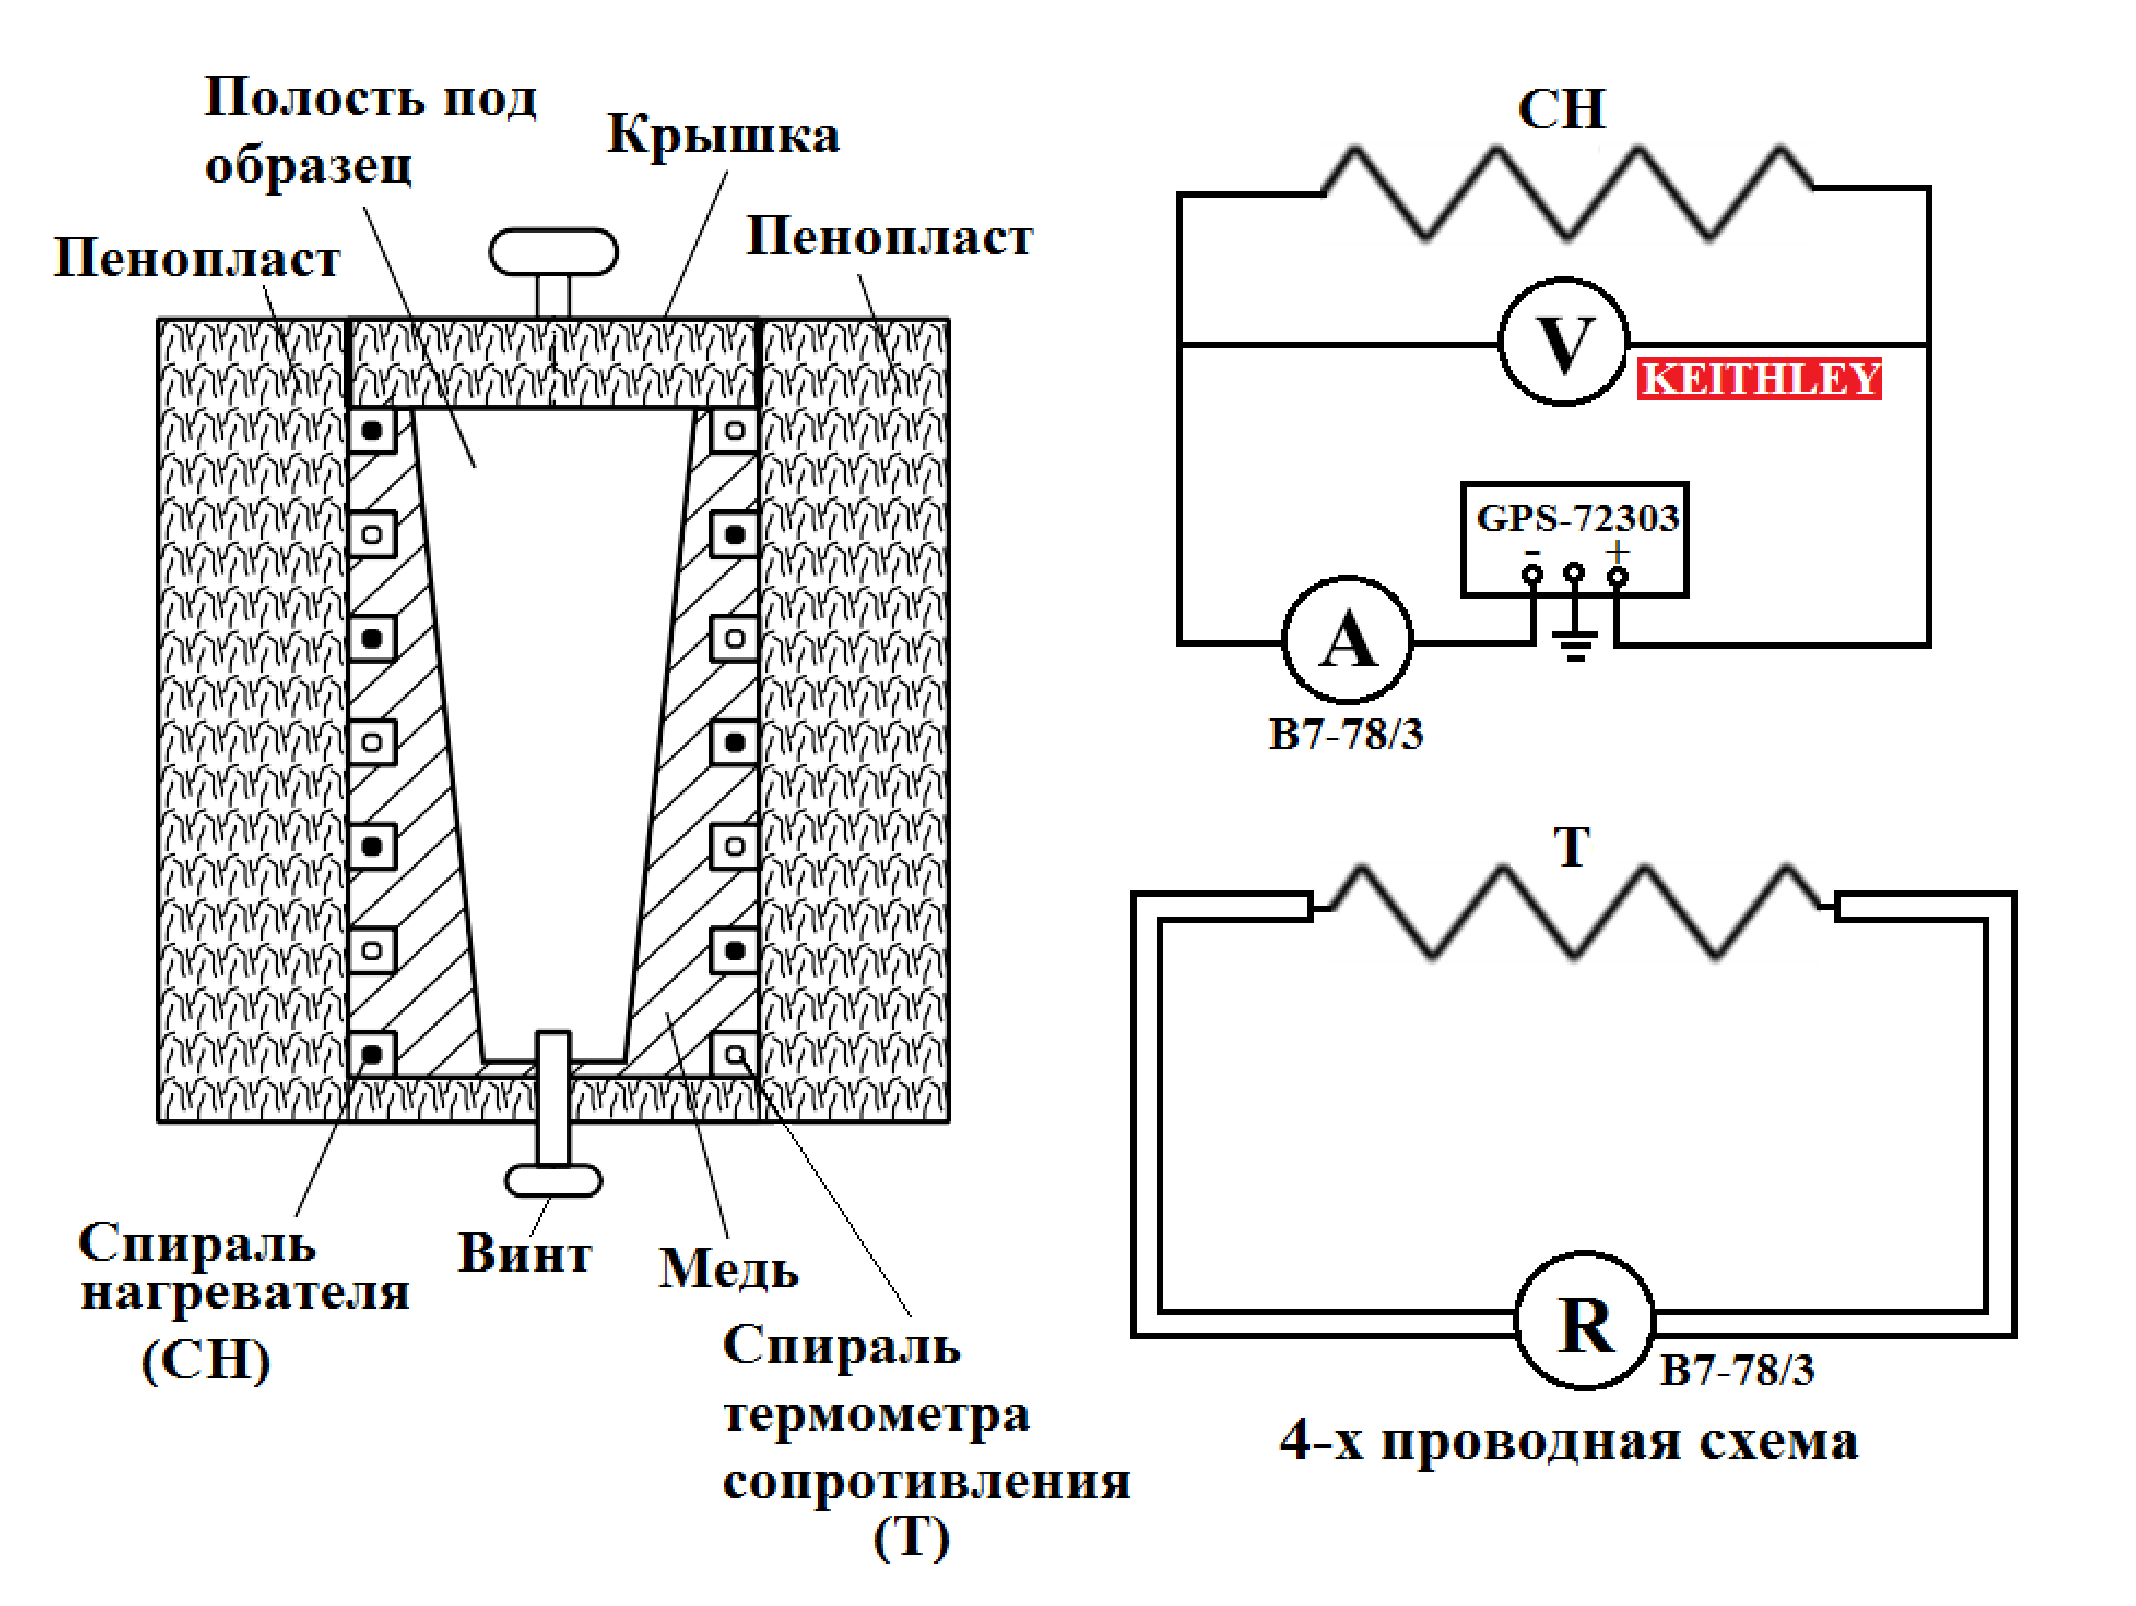
\includegraphics[width=0.6\textwidth]{schema_calorimeter.png}
    \caption{Схема устройства калориметра}
    \label{fig:schema}
\end{figure}

\subsection{Методика проведения эксперимента}
Температура измеряется с помощью термометра сопротивления. Сопротивление проводника изменяется с температурой по закону:
\begin{equation}
    R_T = R_{273}(1 + \alpha(T - 273)),
    \label{eq:resistance}
\end{equation}
где $R_T$ – сопротивление термометра при температуре $T$, $R_{273}$ – сопротивление при $0^\circ$C, $\alpha$ – температурный коэффициент сопротивления.

Выразим $R_{273}$ через измеренное значение $R_k$ – сопротивление термометра при комнатной температуре. Из \eqref{eq:resistance} имеем:
\begin{equation}
    R_{273} = \frac{R_k}{1 + \alpha(T_k - 273)}.
    \label{eq:R273}
\end{equation}
Подставляя \eqref{eq:R273} в \eqref{eq:resistance}, получаем:
\begin{equation}
    T(R_T) = 273 + \frac{R_T}{\alpha R_k} [1 + \alpha(T_k - 273)] - \frac{1}{\alpha}.
    \label{eq:T_from_R}
\end{equation}
Формула \eqref{eq:T_from_R} позволяет пересчитать кривые $R_{\text{нагр}}(t)$ и $R_{\text{охл}}(t)$ в кривые $T_{\text{нагр}}(t)$ и $T_{\text{охл}}(t)$. Температурный коэффициент сопротивления меди равен $\alpha = 4.28 \times 10^{-3}$ K$^{-1}$.

При $T_k(t) = T_k = \text{const}$ из уравнения \eqref{eq:diff} для процесса охлаждения:
\begin{equation}
    C dT_{\text{охл}} = -\lambda[T_{\text{охл}} - T_k] dt.
    \label{eq:cool_diff}
\end{equation}
Разделяя переменные и интегрируя, получаем:
\begin{equation}
    T_{\text{охл}}(t) = (T_0 - T_k) e^{-\frac{\lambda}{C} t} + T_k,
    \label{eq:cool_exp}
\end{equation}
где $T_0$ – начальная температура. Уравнение \eqref{eq:cool_exp} линеаризуется в координатах $(\ln(T_{\text{охл}} - T_k), t)$.

Для процесса нагревания при $T_k = \text{const}$:
\begin{equation}
    T_{\text{нагр}}(t) = \frac{P}{\lambda} \left(1 - e^{-\frac{\lambda}{C} t}\right) + T_k.
    \label{eq:heat_exp}
\end{equation}

При нестабильной комнатной температуре целесообразно использовать дифференциальный метод. В частности, в точке пересечения кривой нагревания с уровнем комнатной температуры:
\begin{equation}
    C = \frac{P}{(dT_{\text{нагр}}/dt)_{T=T_k}}.
    \label{eq:diff_C}
\end{equation}

Другой способ — использование производных в одной и той же температуре на кривых нагревания и охлаждения. Обозначим $A = (dT/dt)_{\text{нагр}}$ и $B = (dT/dt)_{\text{охл}}$ при $T_{\text{нагр}}(t_1) = T_{\text{охл}}(t_2) = T$. Тогда:
\begin{equation}
    \lambda = \frac{P}{(T - T_{k2})(1 - A/B) + T_{k2} - T_{k1}}, \quad
    C = \frac{P}{A - B + A \frac{T_{k1} - T_{k2}}{T - T_{k1}}}.
    \label{eq:diff_lambda_C}
\end{equation}
При равенстве комнатных температур ($T_{k1} = T_{k2} = T_k$) формулы упрощаются:
\begin{equation}
    \lambda = \frac{P}{(T - T_k)(1 - A/B)}, \quad
    C = \frac{P}{A - B}.
    \label{eq:diff_simple}
\end{equation}

\section{Проведение измерений}

\subsection{Хронология эксперимента}
По данным лабораторного журнала:
\begin{itemize}
    \item 10:40 – начало роста температуры после предварительного охлаждения.
    \item 10:46 – включение нагревателя без образца.
    \item 11:06 – выключение нагревателя.
    \item 11:20 – начало охлаждения.
    \item 11:26 – начало роста температуры.
    \item 11:31 – включение нагревателя с образцом алюминия.
    \item 11:50 – выключение нагревателя.
    \item 12:08 – начало охлаждения.
    \item 12:18 – включение нагревателя с образцом железа.
    \item 12:25 – выключение нагревателя.
\end{itemize}

\subsection{Проведение измерений}

\subsubsection{Охлаждение калориметра}
В калориметр помещается предварительно охлаждённый конус. Спустя 4 минуты после начала медленного роста температуры в калориметре, конус извлекается, и выдерживается ещё 4 минуты. В результате калориметр охлаждается примерно на 5 $^\circ$C ниже комнатной температуры.

\subsubsection{Нагрев пустого калориметра}
Нагреватель включается. После того как температура в калориметре превысила комнатную на 9 $^\circ$C, цепь нагревателя отключается.

\subsubsection{Охлаждение пустого калориметра}
Продолжается наблюдение за изменением температуры. После снижения температуры на 2 градуса относительно максимального значения, начинается подготовка к измерению теплоёмкости калориметра с исследуемым образцом.

\subsubsection{Повторное охлаждение калориметра}
Калориметр снова охлаждается до температуры на 5 $^\circ$C ниже комнатной. В калориметр помещается исследуемый образец, и процедуры нагрева и охлаждения повторяются.

\subsubsection{Исследуемые образцы}
Измерения проводятся для образцов из алюминия и железа. Массы образцов:
\begin{equation}
    m_{\text{Al}} = (294.1 \pm 0.5) \text{ г}, \qquad m_{\text{Fe}} = (293.2 \pm 0.5) \text{ г}.
\end{equation}

\subsubsection{Завершение измерений}
Запись данных в программе останавливается, файлы с результатами сохраняются.

\section{Обработка результатов}

\subsection{Идентификация кривых}
Общий график зависимости температуры от времени представлен на рис. \ref{fig:full}. Сопоставление временных интервалов:

\begin{table}[H]
    \centering
    \begin{tabular}{|l|c|c|}
        \hline
        \textbf{Процесс} & \textbf{Начало, с} & \textbf{Конец, с} \\
        \hline
        $T_{\text{нагр1}}(t)$ – нагрев пустого калориметра & 1000 & 2500 \\
        $T_{\text{охл1}}(t)$ – охлаждение пустого калориметра & 2600 & 3700 \\
        $T_{\text{нагр2}}(t)$ – нагрев с алюминием & 4800 & 6000 \\
        $T_{\text{охл2}}(t)$ – охлаждение с алюминием & 6300 & 6900 \\
        $T_{\text{нагр3}}(t)$ – нагрев с железом & 7800 & 8600 \\
        $T_{\text{охл3}}(t)$ – охлаждение с железом & 8800 & 9300 \\
        \hline
    \end{tabular}
    \caption{Сопоставление временных интервалов экспериментальным кривым}
    \label{tab:times}
\end{table}

Изменение комнатной температуры за время эксперимента не превышало 2 К, что позволяет использовать интегральный метод обработки.

\subsection{Теплоёмкость пустого калориметра}
Для пустого калориметра построена кривая охлаждения в координатах $(\ln(T_{\text{охл}} - T_k), t)$ (рис. \ref{fig:cool_empty}). Начальный нелинейный участок исключён. По методу наименьших квадратов определён угловой коэффициент прямой, который согласно \eqref{eq:cool_exp} равен $-\lambda/C$.

\begin{figure}[H]
    \centering
    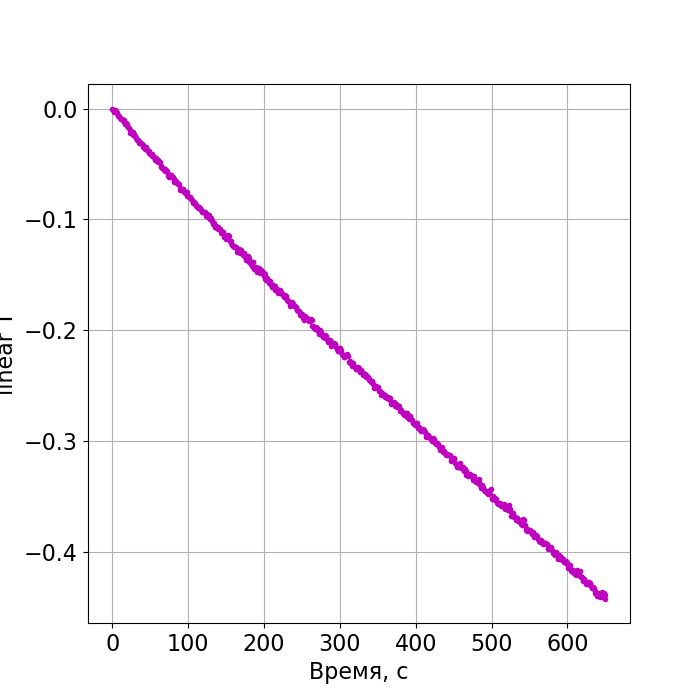
\includegraphics[width=0.7\textwidth]{cooling_empty.png}
    \caption{Кривая охлаждения пустого калориметра в полулогарифмических координатах}
    \label{fig:cool_empty}
\end{figure}

Результат:
\begin{equation}
    \frac{\lambda}{C} = (33 \pm 2) \times 10^{-5} \text{ c}^{-1}.
\end{equation}

Из кривой нагревания по формуле \eqref{eq:heat_exp} определён параметр $\lambda$:
\begin{equation}
    \lambda = (0.24 \pm 0.02) \ \frac{\text{Вт}}{\text{К} \cdot \text{с}}.
\end{equation}
Теплоёмкость пустого калориметра:
\begin{equation}
    C_{\text{кал}} = \lambda \Big/ \frac{\lambda}{C} = (0.73 \pm 0.07) \ \frac{\text{кДж}}{\text{К}}.
\end{equation}

\subsection{Теплоёмкость алюминия}
Аналогично для системы «калориметр + алюминий» получены следующие значения. Кривая охлаждения представлена на рис. \ref{fig:cool_al}.

\begin{figure}[H]
    \centering
    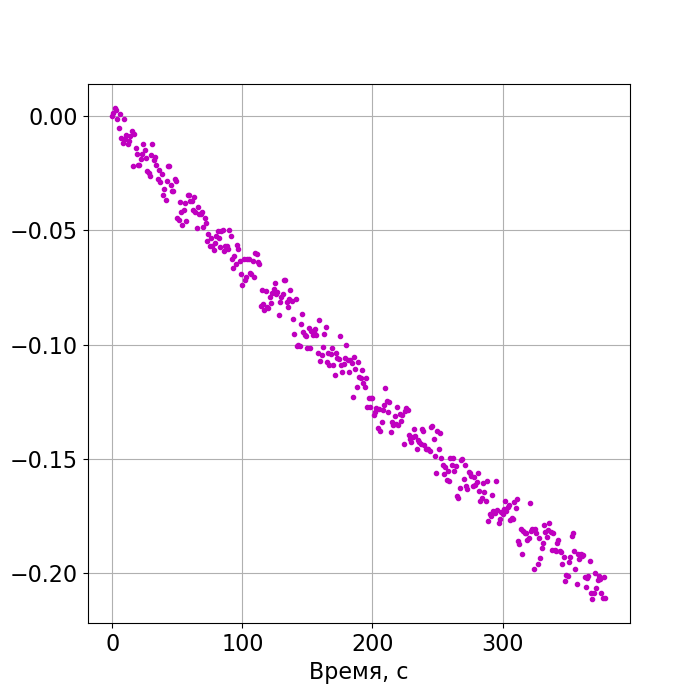
\includegraphics[width=0.7\textwidth]{cooling_aluminum.png}
    \caption{Кривая охлаждения калориметра с алюминиевым образцом в полулогарифмических координатах}
    \label{fig:cool_al}
\end{figure}

\begin{equation}
    \frac{\lambda}{C_{\text{сум}}} = (22 \pm 4) \times 10^{-5} \text{ c}^{-1}, \qquad
    \lambda = (0.21 \pm 0.04) \ \frac{\text{Вт}}{\text{К} \cdot \text{с}}.
\end{equation}
Суммарная теплоёмкость системы:
\begin{equation}
    C_{\text{сум,Al}} = \lambda \Big/ \frac{\lambda}{C_{\text{сум}}} = (0.95 \pm 0.18) \ \frac{\text{кДж}}{\text{К}}.
\end{equation}
Теплоёмкость алюминиевого образца:
\begin{equation}
    C_{\text{Al}} = C_{\text{сум,Al}} - C_{\text{кал}} = (0.22 \pm 0.19) \ \frac{\text{кДж}}{\text{К}}.
\end{equation}
Удельная теплоёмкость алюминия:
\begin{equation}
    c_{\text{Al}} = \frac{C_{\text{Al}}}{m_{\text{Al}}} = (0.75 \pm 0.65) \ \frac{\text{кДж}}{\text{кг} \cdot \text{К}}.
\end{equation}

\subsection{Теплоёмкость железа}
Аналогично для системы «калориметр + железо» получены следующие значения. Кривая охлаждения представлена на рис. \ref{fig:cool_fe}.

\begin{figure}[H]
    \centering
    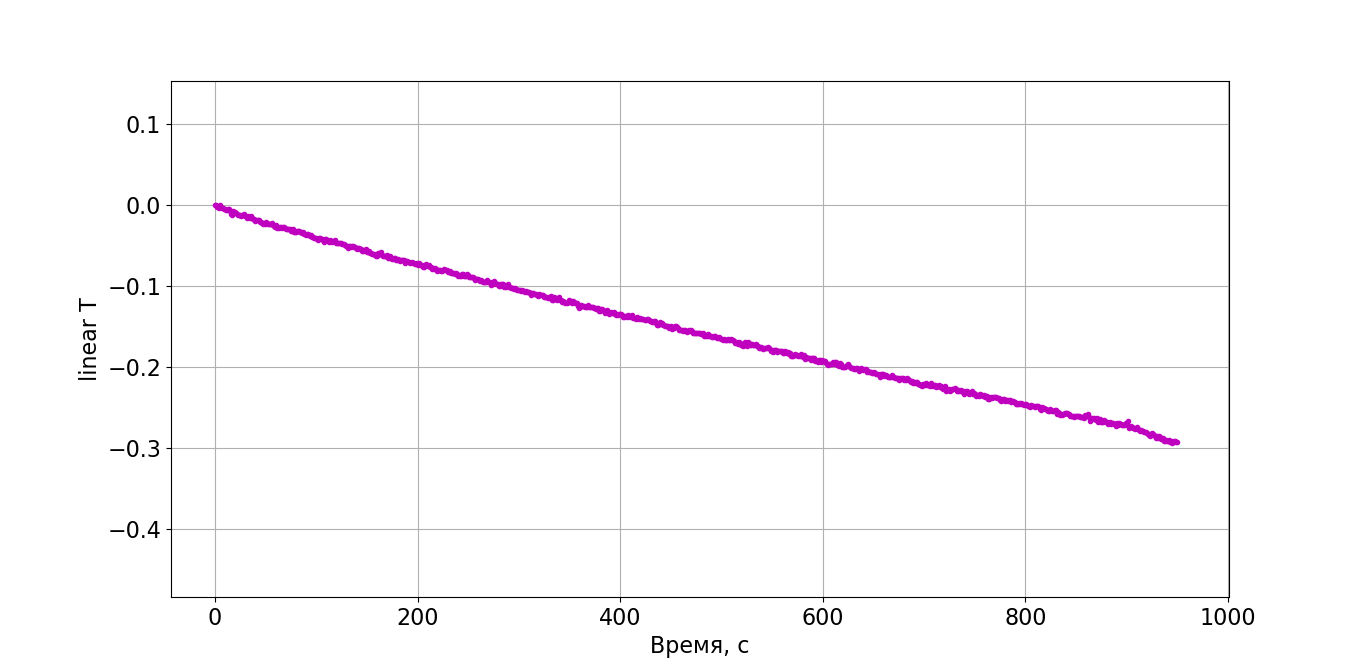
\includegraphics[width=0.7\textwidth]{cooling_iron.png}
    \caption{Кривая охлаждения калориметра с железным образцом в полулогарифмических координатах}
    \label{fig:cool_fe}
\end{figure}

\begin{equation}
    \frac{\lambda}{C_{\text{сум}}} = (28 \pm 5) \times 10^{-5} \text{ c}^{-1}, \qquad
    \lambda = (0.20 \pm 0.04) \ \frac{\text{Вт}}{\text{К} \cdot \text{с}}.
\end{equation}
Суммарная теплоёмкость системы:
\begin{equation}
    C_{\text{сум,Fe}} = \lambda \Big/ \frac{\lambda}{C_{\text{сум}}} = (0.71 \pm 0.16) \ \frac{\text{кДж}}{\text{К}}.
\end{equation}
Теплоёмкость железного образца:
\begin{equation}
    C_{\text{Fe}} = C_{\text{сум,Fe}} - C_{\text{кал}} = (-0.02 \pm 0.18) \ \frac{\text{кДж}}{\text{К}}.
\end{equation}
В пределах погрешности значение близко к нулю, что указывает на необходимость более аккуратного вычитания. Для корректной оценки воспользуемся дифференциальным методом.

\subsection{Теплоёмкость пустого калориметра дифференциальным методом}
По формуле \eqref{eq:diff_C} в момент, когда температура при нагреве равна комнатной ($dT = 0.5$ К):
\begin{equation}
    C_{\text{кал}} = (0.70 \pm 0.15) \ \frac{\text{кДж}}{\text{К}}.
\end{equation}

По формуле \eqref{eq:diff_simple} при $T_{\text{нагр}}(t) = T_{\text{охл}}(t) = 304.5$ К:
\begin{equation}
    C_{\text{кал}} = (0.75 \pm 0.18) \ \frac{\text{кДж}}{\text{К}}.
\end{equation}

\subsection{Теплоёмкость алюминия дифференциальным методом}

По формуле \eqref{eq:diff_C}:
\begin{equation}
    C_{\text{Al}} = (0.23 \pm 0.20) \ \frac{\text{кДж}}{\text{К}}, \qquad
    c_{\text{Al}} = (0.78 \pm 0.68) \ \frac{\text{кДж}}{\text{кг} \cdot \text{К}}.
\end{equation}

По формуле \eqref{eq:diff_simple}:
\begin{equation}
    C_{\text{Al}} = (0.20 \pm 0.18) \ \frac{\text{кДж}}{\text{К}}, \qquad
    c_{\text{Al}} = (0.68 \pm 0.61) \ \frac{\text{кДж}}{\text{кг} \cdot \text{К}}.
\end{equation}

\subsection{Теплоёмкость железа дифференциальным методом}

По формуле \eqref{eq:diff_C}:
\begin{equation}
    C_{\text{Fe}} = (0.14 \pm 0.12) \ \frac{\text{кДж}}{\text{К}}, \qquad
    c_{\text{Fe}} = (0.48 \pm 0.41) \ \frac{\text{кДж}}{\text{кг} \cdot \text{К}}.
\end{equation}

По формуле \eqref{eq:diff_simple}:
\begin{equation}
    C_{\text{Fe}} = (0.12 \pm 0.11) \ \frac{\text{кДж}}{\text{К}}, \qquad
    c_{\text{Fe}} = (0.41 \pm 0.38) \ \frac{\text{кДж}}{\text{кг} \cdot \text{К}}.
\end{equation}

\section{Вывод}
Табличные значения удельных теплоёмкостей:
\begin{equation}
    c_{\text{Al}}^{\text{табл}} = 0.902 \ \frac{\text{кДж}}{\text{кг} \cdot \text{К}}, \qquad
    c_{\text{Fe}}^{\text{табл}} = 0.450 \ \frac{\text{кДж}}{\text{кг} \cdot \text{К}}.
\end{equation}

Полученные в работе результаты:
\begin{itemize}
    \item Алюминий: $c_{\text{Al}} = 0.75 \pm 0.65$ (интегральный метод), $c_{\text{Al}} = 0.73 \pm 0.64$ (дифференциальный метод).
    \item Железо: $c_{\text{Fe}} = 0.48 \pm 0.41$ (дифференциальный метод); интегральный метод дал значение, близкое к нулю из-за погрешностей вычитания.
\end{itemize}

Все полученные значения в пределах погрешностей согласуются с табличными данными. Относительные погрешности дифференциального метода выше, что связано с определением производной на малом участке графика, где возрастает влияние приборной погрешности измерения температуры.

Значительная погрешность результатов обусловлена процедурой вычитания теплоёмкости калориметра из суммарной теплоёмкости системы. Поскольку теплоёмкость калориметра в несколько раз превышает теплоёмкость образцов, погрешность при вычитании возрастает до величин, сопоставимых с самими значениями.

В ходе работы были зарегистрированы кривые нагревания и охлаждения пустого калориметра и системы «калориметр + твёрдое тело». Определён коэффициент теплопередачи стенок калориметра. Вычислены теплоёмкость пустого калориметра и удельные теплоёмкости алюминия и железа.

\section{Приложение}

\begin{figure}[H]
    \centering
    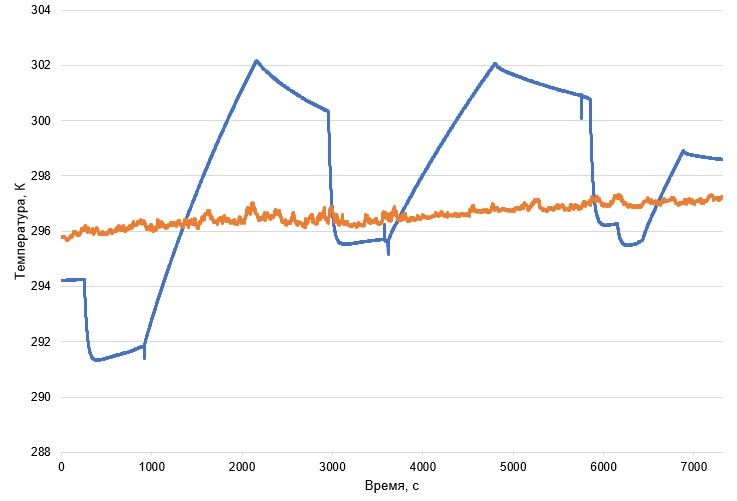
\includegraphics[width=0.9\textwidth]{full_experiment}
    \caption{Температуры калориметра и комнаты за всё время эксперимента}
    \label{fig:full}
\end{figure}

\end{document}